%%%%%%%%%%%%%%%%%%%%%%%%%%%%%%%%%%%%%%%%%%%%%%%%%%%
%% P3: Phenomenology of Particle Physics                         
%%
%% Author:  André Rubbia                   		 
%%
%% Figure 27.18 Precision measurement of the hadronic pole cross-section of the ratio of the hadronic to leptonic width at LEP.
%%
%% This work is licensed under the Creative Commons Attribution 4.0 International License. 
%% To view a copy of this license, visit http://creativecommons.org/licenses/by/4.0/ or 
%% send a letter to Creative Commons, PO Box 1866, Mountain View, CA 94042, USA.
%%
%%%%%%%%%%%%%%%%%%%%%%%%%%%%%%%%%%%%%%%%%%%%%%%%%%%

\documentclass[a4paper,10pt]{article}

\usepackage[T1]{fontenc}
\usepackage[utf8]{inputenc}
\usepackage{lmodern}
\usepackage[labelfont=bf]{caption}
\usepackage{upgreek}

\usepackage{tikz}
\usepackage{pgfplots}
\pgfplotsset{compat=1.17}
\usepgfplotslibrary{ternary}
\usepgfplotslibrary{fillbetween}
\usepgfplotslibrary{external}

\def\d{\mathrm{d}}
\setlength{\oddsidemargin}{-1.0cm}
\setlength{\evensidemargin}{-1.0cm}
\setlength{\textheight}{25cm}
\setlength{\textwidth}{18cm}

\pgfkeys{/pgf/number format/.cd,1000 sep={}}

\begin{document}

%%%%%%%%%%%%%%%%   FIGURE  %%%%%%%%%%%%%%%%%%%%%%%%%%%%%%
\begin{figure}[htb]
 	\centering
%
%%% hadronic pole cross-section
%
\begin{tikzpicture}[scale=1]
\begin{axis}[
    xbar,
    width=7cm,
    height=4cm,
    title={Hadronic pole cross-section},
    xlabel={$\sigma^0_{had}$ [nb]},
    symbolic y coords={ybot,average,OPAL,L3,DELPHI,ALEPH,ytop},
    ytick=data,
    ymin=ybot,ymax=ytop,
    xmin=41.4, xmax=42.115,
    legend pos=north east,
]
\addplot[
    color=blue,only marks,
    mark=*,
        error bars/.cd,
    x dir=both, x explicit
    ]
    coordinates {
    (41.559,ALEPH)+-(0.058,0)
    (41.578,DELPHI)+-(0.069,0)
    (41.535,L3)+-(0.055,0)
    (41.501,OPAL)+-(0.055,0)
    (41.541,average)+-(0.037,0)
};
    \draw[gray,fill,fill opacity=0.2] (axis cs:41.503,ybot) rectangle (axis cs:41.577,ytop);
    \node at  (axis cs:41.88,ALEPH) {$41.559\pm 0.057$~\cite{Barate:1999ce}};
    \node at  (axis cs:41.88,DELPHI) {$41.578\pm 0.069$~\cite{Abreu:2000mh}};
    \node at  (axis cs:41.88,L3) {$41.535\pm 0.055$~\cite{Acciarri:2000ai}};
    \node at  (axis cs:41.88,OPAL) {$41.501\pm 0.055$~\cite{Abbiendi:2000hu}};
    \node at  (axis cs:41.88,average) {$41.541\pm 0.037$};
\end{axis}
\end{tikzpicture}
%
\hspace{1cm}
%
%%% ratio hadronic to leptonic
%
\begin{tikzpicture}[scale=1]
\begin{axis}[
    xbar,
    width=7cm,
    height=4cm,
    title={Hadronic to leptonic width},
    xlabel={Ratio $R_\ell = \Gamma_{had}/\Gamma_{\ell}$},
    symbolic y coords={ybot,average,OPAL,L3,DELPHI,ALEPH,ytop},
    ytick=data,
    ymin=ybot,ymax=ytop,
    xmin=20.65, xmax=21.3,
    legend pos=north east,
]
\addplot[
    color=blue,only marks,
    mark=*,
        error bars/.cd,
    x dir=both, x explicit
    ]
    coordinates {
    (20.729,ALEPH)+-(0.039,0)
    (20.730,DELPHI)+-(0.060,0)
    (20.809,L3)+-(0.060,0)
    (20.822,OPAL)+-(0.044,0)
    (20.767,average)+-(0.025,0)
};
    \draw[gray,fill,fill opacity=0.2] (axis cs:20.742,ybot) rectangle (axis cs:20.792,ytop);
    \node at  (axis cs:21.1,ALEPH) {$20.729\pm 0.039$~\cite{Barate:1999ce}};
    \node at  (axis cs:21.1,DELPHI) {$20.730\pm 0.060$~\cite{Abreu:2000mh}};
    \node at  (axis cs:21.1,L3) {$20.809\pm 0.060$~\cite{Acciarri:2000ai}};
    \node at  (axis cs:21.1,OPAL) {$20.822\pm 0.044$~\cite{Abbiendi:2000hu}};
    \node at  (axis cs:21.1,average) {$20.767\pm 0.025$};
\end{axis}
\end{tikzpicture}
		\caption{Precision measurement of the hadronic pole cross-section
		of the ratio of the hadronic to leptonic width at LEP.
		The average value is from the PDG.}
\end{figure}
%
%%%%%%%%%%%%%%%%   END FIGURE  %%%%%%%%%%%%%%%%%%%%%%%%%%%%%%
%

\begin{thebibliography}{99}
\bibitem{Barate:1999ce}
R.~Barate {\em et~al.}, ``{Measurement of the Z resonance parameters at LEP},''
  {\em Eur. Phys. J. C}, vol.~14, pp.~1--50, 2000.

\bibitem{Abreu:2000mh}
P.~Abreu {\em et~al.}, ``{Cross-sections and leptonic forward backward
  asymmetries from the Z0 running of LEP},'' {\em Eur. Phys. J. C}, vol.~16,
  pp.~371--405, 2000.

\bibitem{Acciarri:2000ai}
M.~Acciarri {\em et~al.}, ``{Measurements of cross-sections and forward
  backward asymmetries at the $Z$ resonance and determination of electroweak
  parameters},'' {\em Eur. Phys. J. C}, vol.~16, pp.~1--40, 2000.

\bibitem{Abbiendi:2000hu}
G.~Abbiendi {\em et~al.}, ``{Precise determination of the Z resonance
  parameters at LEP: 'Zedometry'},'' {\em Eur. Phys. J. C}, vol.~19,
  pp.~587--651, 2001.
\end{thebibliography}

\end{document}
